\documentclass[USenglish]{article}

\usepackage[utf8]{inputenc}
\usepackage{xparse}
\usepackage[big,online]{dgruyter}
\usepackage{lmodern}
\usepackage{microtype}
\usepackage[authoryear,round,sort&compress]{natbib}
\usepackage{graphicx}
\usepackage{booktabs}
\usepackage{multirow}
\usepackage{array}
\usepackage{longtable}
\usepackage{amsmath}

\theoremstyle{dgthm}
\newtheorem{theorem}{Theorem}
\newtheorem{corollary}{Corollary}
\newtheorem{proposition}{Proposition}
\newtheorem{lemma}{Lemma}

\theoremstyle{dgdef}
\newtheorem{definition}{Definition}
\newtheorem{example}{Example}
\newtheorem{remark}{Remark}

\begin{document}

%%%--------------------------------------------%%%
\articletype{Research Article}
\received{Month DD, YYYY}
\revised{Month DD, YYYY}
\accepted{Month DD, YYYY}
\journalname{Journal of Quantitative Analysis in Sports}
\journalyear{YYYY}
\journalvolume{XX}
\journalissue{X}
\startpage{1}
\aop
\DOI{10.1515/jqas-YYYY-XXXX}
%%%--------------------------------------------%%%

\title{Predicting NFL Head Coach Dismissal at the Time of Hire: A Firing-Aware Survival Analysis}
\runningtitle{Predicting NFL Head Coach Dismissal}

% Author information removed for blind peer review
%\author*[1]{Jon Williamson}
%\runningauthor{J.~Williamson}
%\affil[1]{\protect\raggedright
%Des Moines, Iowa, e-mail: jon@williamsonconsultinggroup.com}

\abstract{Each NFL off-season brings a wave of head coaching changes, and a coach's tenure is the clearest public measure of whether the hire worked. Yet whether a hire will end in firing is poorly understood the moment the contract is signed. Prior work has largely modeled the in-season firing decision from results posted during the tenure, leaving open how much is foreseeable on hiring day. We recast the problem as a firing-aware survival analysis. Across 371 head coaching stints (1970--2025), we model the time from hire to firing, treating voluntary departures as a competing risk and active coaches as censored, using only pre-hire information. A cause-specific Cox proportional-hazards model, benchmarked against parametric and gradient-boosted alternatives and fit on features chosen by Cox-native stability selection, proves only modestly predictive: a Harrell concordance of 0.602 (95\% CI [0.560, 0.645]) and an integrated Brier score of 0.176. The one robust signal is not the coach's credentials but the structure of the hire: internal promotions face a higher firing hazard than external hires (HR 1.52), with weaker effects from age at hire and prior-unit yards-per-play efficiency. The broad performance record that hiring processes scrutinize, points, yards, and turnovers, forecasts dismissal no better than chance.}

\keywords{survival analysis, head coach, National Football League, Cox proportional hazards, competing risks}

\maketitle

\section{Introduction}

Hiring a head coach is one of the most consequential personnel decisions an NFL franchise makes, and the record shows how often it is undone. Of the 371 stints we study in the modern era (1970 onward), 84\% ended in an involuntary parting, and the median coach survived only four seasons before being fired. Teams pour weeks of interviews, scheme presentations, and background checks into the choice, sometimes enlisting outside search consultants \citep{perez2025, brandt2026}, yet reversals are common enough to raise a basic question: at the moment a coach is hired, before a single game has been played, how foreseeable is the eventual firing from the information the team actually has in hand?

Research on NFL coaching turnover consistently finds that dismissal is driven by a coach's performance in the job \citep{allen2012, salaga2020, foreman2019, farnell2021}. As we detail in Section~\ref{sec:litreview}, however, these studies share a structural approach: they explain dismissal using covariates realized \emph{during} the tenure, such as team-season win percentage, player fines and penalties, or performance relative to expectations. These models answer a retrospective question, what about a tenure, once it has unfolded, is associated with firing, and their recurring answer, that losing leads to firing, offers little to a team deciding whom to hire.

The prospective version of this question is harder: using only what can be observed when the contract is signed, how much of an eventual firing is already foreseeable? If pre-hire signal is strong, dismissals reflect foreseeable mismatches that sharper evaluation could reduce. If it is weak, the outcome is determined largely by events that unfold only after the contract is signed. The answer bears both on how franchises allocate their evaluation effort and on the broader debate over whether coaching changes accomplish what teams intend \citep{bryson2024}.

We frame NFL head coach dismissal as a pre-hire, firing-aware, competing-risks forecasting problem, separating the foreseeable component of the outcome from the larger part realized only after the hire. We then use that framing to ask how much of an eventual dismissal is written into the information available on hiring day, and where any foreseeable signal resides.

\section{Literature Review}
\label{sec:litreview}

\subsection{Determinants of NFL head coach dismissal}

The economics of NFL coaching turnover has received sustained attention, and its consistent message is that dismissal is driven by performance. \citet{allen2012} estimate probit models of turnover over 1979--2006 and exploit the early-1990s introduction of the salary cap and free agency as a natural experiment, finding that both the probability of dismissal and the weight placed on talent and on-field results increased once the cap made measurable performance more decisive. \citet{salaga2020} apply survival methods to 208 head coach employment spells from 1985 to 2018, but model dismissal from on-field performance accumulated \emph{during} the tenure; they conclude that firing is driven largely by raw, and to a lesser degree relative, in-season results rather than by anything known at the time of hire. \citet{foreman2019} fit a hazard model to 505 team-seasons (2000--2015) and show that player deviance, measured through fines, penalties, and off-field legal incidents, raises the dismissal hazard. \citet{farnell2021} examine the full coaching hierarchy and find that young, experienced, well-performing coordinators tend to be promoted, while older and poorly performing coaches tend to be fired, with race playing little role in either decision.

What unites these studies is that every covariate is realized \emph{during} the tenure, so they characterize which in-season outcomes accompany a firing rather than what, if anything, foreshadows it at the time of hire.

\subsection{Survival modeling of managerial tenure and the case for Cox}
\label{sec:litcox}

A coaching spell is naturally a time-to-event outcome: it has a start, an end that is either observed (a departure) or not yet observed (an ongoing tenure), and a duration whose distribution is the quantity of interest. Survival analysis is the standard framework for such data for several reasons. It models the full time-to-event distribution, the hazard of firing at each point in a tenure, rather than collapsing the outcome to whether a coach was fired or to an average tenure length; it accommodates right-censoring, the coaches still employed at the end of the study window, so those incomplete spells inform the fit instead of being discarded as a regression on observed tenure would require; and it expresses covariate effects as shifts in the timing of the event, not merely its occurrence. The framework has been used across sports management. \citet{gilfix2020} study Major League Soccer manager longevity and find that performance relative to predecessors, league context, and age at hire all affect tenure duration. \citet{salaga2020} fit Cox survival models to 208 NFL coaching spells over 1985--2018, but, as in the dismissal studies above, their covariates are realized during the tenure (raw and relative on-field performance) rather than fixed at hire.

Within survival analysis, the Cox proportional-hazards model \citep{cox1972} is among the most widely used time-to-event models across the empirical sciences, and we adopt it as our primary model. It is semi-parametric, leaving the baseline hazard (the shape of firing risk over the course of a tenure) unspecified, which avoids committing in advance to a parametric clock for when coaches are fired; its coefficients exponentiate into interpretable hazard ratios, which suits a study whose substantive interest is in \emph{which} factors foreshadow firing; and it is the established choice in the cognate sports-management literature \citep{salaga2020, gilfix2020}, keeping our results comparable to prior work. Whether this interpretability costs any accuracy is an empirical question we take up in Section~\ref{sec:models}.

\subsection{Prediction from pre-hire information}

Methodologically, our framing is closest to work that forecasts sports outcomes from information available before the outcome is realized. \citet{wolfson2011} forecast NFL quarterback career success from pre-draft observables and find that much of the variation in future performance is driven by factors not observable in advance, a forecasting problem structurally similar to the one we pose. \citet{roach2016} relates early-career team performance to prior head coaching experience and other pre-hire predictors and finds no positive association. Other NFL machine-learning work predicts within-game or within-season outcomes \citep{lock2014, david2011}, a different problem from forecasting at the time of hire.

\section{Methods}

We predict the time from hire to firing for NFL head coaches using only information available at the time of hire. Raw coaching histories and team performance statistics are scraped from Pro-Football-Reference.com \citep{pfr} and supplemented with team and roster data covering 1970--2024. All modeling is performed in Python with \texttt{scikit-learn} \citep{pedregosa2011} and the \texttt{lifelines} survival library \citep{davidsonpilon2019}.

\subsection{Population and outcome}

The analysis covers 371 non-interim head coaching stints held by 264 distinct coaches who were hired between 1970 and 2025; 86 coaches account for more than one stint, and four (Bill Parcells, Pete Carroll, Chuck Knox, and Marty Schottenheimer) appear four times each. Because survival analysis treats an ongoing tenure as a right-censored observation rather than a missing outcome, we retain every coach still employed at the data boundary, including recent hires whose tenures have not yet concluded. Mid-season interim appointments that did not convert into a non-interim role are excluded, and interim appointments later retained on a non-interim basis are anchored to the season in which that tenure began. The duration of a stint is the number of seasons the coach held the position. As a check that dismissal is a meaningful outcome rather than noise, Appendix~\ref{app:winrate} relates tenure length to regular-season winning percentage, which rises across short, medium, and long stints (Kruskal--Wallis $p < 10^{-30}$).

\subsubsection{Competing-risks event coding}
\label{sec:coding}

We distinguish three terminal states for each stint, summarized in Table~\ref{tab:events}. The event of interest is \emph{involuntary non-retention}: a firing, a forced resignation, a face-saving ``mutual'' parting, or a performance-driven non-renewal. The two complementary states are a \emph{voluntary-while-viable} departure, which we treat as a competing event, and a tenure still ongoing at the data boundary, which is administratively censored.

Classifying departures is difficult because the labels organizations attach to a coaching change are unreliable. A fired coach is routinely described as having ``stepped down,'' and a ``mutual parting'' is frequently a dismissal in all but name. We therefore adopt a conservative, asymmetric protocol. Involuntary non-retention is the \emph{default}: a stint is coded as a firing unless we found positive, documented evidence that the coach left on his own terms while still employable. A departure is coded as voluntary, and hence censored, only when it falls into one of three pre-specified categories, each established from contemporaneous reporting:
\begin{quote}
\begin{enumerate}
\item[(A)] the coach left to take another head coaching position while still wanted by the incumbent team;
\item[(B)] the coach retired while still successful and retained (a ``retirement on top''); or
\item[(C)] the coach departed for documented health, family, or other non-football reasons.
\end{enumerate}
\end{quote}
Each of the 27 voluntary departures was researched and adjudicated individually, recording a one-line justification, a confidence level, and a source; the full classification, with category and justification, is given in Appendix~\ref{app:nonfiring}. The remaining 32 non-firings are coaches still active at the data boundary (the 2025 season). The default-to-firing rule is deliberately conservative against cosmetic exit language: where reporting was ambiguous, we coded the exit as a firing rather than credit an unverified voluntary narrative.

\begin{table}[!ht]
\caption{Competing-risks coding of the 371 head coaching stints. The firing hazard treats voluntary departures and active coaches as censored; the cumulative incidence function (Section~\ref{sec:cif}) treats voluntary departure as a competing event.}
\label{tab:events}
\small
\begin{tabular}{llcc}
\toprule
Code & Terminal state & Count & Share \\
\midrule
1 (event) & Involuntary non-retention (firing) & 312 & 84.1\% \\
2 (competing) & Voluntary-while-viable departure & 27 & 7.3\% \\
0 (censored) & Active at data boundary & 32 & 8.6\% \\
\midrule
& Total & 371 & 100\% \\
\bottomrule
\end{tabular}
\end{table}

The two quantities we estimate call for voluntary exits to be handled in two different ways, which is standard in competing-risks analysis \citep{austin2016}. For absolute risk, a voluntary departure is a competing event: such a stint can never subsequently end in a firing, so censoring it na\"ively would overstate the cumulative firing incidence (Section~\ref{sec:cif}). For the cause-specific hazard, which asks what raises the rate of firing among coaches still at risk of it, the correct handling is the reverse, with voluntary departures and active coaches both censored. Each quantity is therefore estimated under the censoring convention appropriate to it.

\subsection{Pre-hire features}

The analysis uses 74 pre-hire features for each hire, all fixed at the time of hire and organized into eight families on two tiers: the coach being hired and the situation he inherits (Table~\ref{tab:feature_categories}). They are constructed so that each underlying construct enters once: where several measures capture the same construct, for instance a team rating and the components that sum to it, a single representative is kept (Section~\ref{sec:selection}). The description that follows, and the formal definitions in Appendix~\ref{app:features}, concern this feature set.

\begin{table}[!ht]
\caption{The 74 pre-hire features on two tiers: attributes of the coach being hired, and attributes of the situation he inherits. All values are measured at or before the hire date; Appendix~\ref{app:features} defines every feature.}
\label{tab:feature_categories}
\small
\begin{tabular}{ll}
\toprule
Family & Description \\
\midrule
\multicolumn{2}{@{}l}{\emph{The coach (who is hired)}}\\
Core experience & Age at hire, prior HC stints, years by coaching level and role \\
Career structure & Employer history, role and side exposure, internal-hire indicator \\
Prior unit performance & Pooled, orientation-signed unit statistics from prior roles (App.~\ref{app:unitstats}) \\
Recent form & Percentile and trajectory of the coach's recent unit and team performance \\
\addlinespace
\multicolumn{2}{@{}l}{\emph{The situation (what is inherited)}}\\
Hiring-team results & Recent record, scoring, yards, turnovers, and playoff appearances \\
Inherited team quality & Team rating (SRS) components and schedule strength \\
Inherited roster & Roster and starter value, age, experience, retention, draft capital \\
Organizational instability & Predecessor tenure, distinct HCs in the prior decade \\
\bottomrule
\end{tabular}
\end{table}

Several inherited-quality features use the Simple Rating System (SRS), reported by Pro-Football-Reference \citep{pfr}, which rates a team by its average point margin adjusted for strength of schedule and expresses it in points per game relative to a league-average team. Its offensive and defensive components divide that rating into points generated and points prevented.

\subsubsection{Pooled unit representation}

A coach accumulates performance statistics in several prior roles (offensive coordinator, defensive coordinator, head coach). Rather than maintain four parallel statistical blocks (one per role and side), which leaves most cells empty for any individual coach, we pool a coach's prior role-seasons into a single oriented \emph{unit} block of 33 statistics (itemized in Appendix~\ref{app:unitstats}). Each season the coach worked is mapped to the side of the ball that role controlled, and the contribution is signed so that larger values are always better: an offensive coordinator's season contributes its team's offensive output; a defensive coordinator's season contributes the suppression of the opposing offense; a head coach's season contributes both. Turnovers and penalties are sign-flipped so that fewer is better. Per-season values are normalized relative to that season's league distribution,
\begin{equation}
z_{i,s,t} = \frac{x_{i,s,t} - \mu_{s,t}}{\sigma_{s,t}},
\label{eq:zscore}
\end{equation}
where $x_{i,s,t}$ is statistic $s$ for coach $i$'s relevant unit in season $t$ and $\mu_{s,t}, \sigma_{s,t}$ are the league mean and standard deviation that season, then pooled across all of the coach's qualifying role-seasons. This makes a coach who ran a top-decile offense in 1985 comparable to one who did so in 2020 and lets a coach's full body of work, rather than one role in isolation, inform the prediction.

\subsubsection{Missing data}

The pooled unit representation just described removes the structural emptiness that a role-by-role layout would otherwise create: a coach's qualifying role-seasons all feed one oriented block, rather than leaving parallel offensive, defensive, and head coaching blocks empty for a coach who never held one of those roles. Where the relevant information is itself a binary career fact, such as whether a coach ever served as an NFL coordinator on a given side, it is encoded directly as an indicator, so that ``never held the role'' is represented as information rather than as a value to be guessed. The missingness that remains is not scattered at random but concentrated in the advanced efficiency and drive statistics the league only began recording in the 1990s, so it falls almost entirely on coaches whose qualifying seasons predate those measures; it is imputed by truncated singular value decomposition, approximating the feature matrix by a low-rank factorization $\mathbf{X} \approx \mathbf{U}\boldsymbol{\Sigma}\mathbf{V}^\top$ re-fit within each resample on training data alone (Section~\ref{sec:eval}).

\subsection{Survival models}
\label{sec:models}

Our primary model is the Cox proportional-hazards model \citep{cox1972}, which specifies the firing hazard for stint $i$ as
\begin{equation}
\lambda_i(t \mid \mathbf{x}_i) = \lambda_0(t)\,\exp(\mathbf{x}_i^\top \boldsymbol{\beta}),
\label{eq:cox}
\end{equation}
leaving the baseline hazard $\lambda_0(t)$ unspecified. For predictive evaluation the model is fit with elastic-net regularization, whose penalty strength and $\ell_1$ mixing are chosen by coach-level cross-validated concordance over a grid (penalizer $0.5$ and $\ell_1$ ratio $0.25$ at the optimum; Appendix~\ref{app:hyperparameters}); regularization stabilizes estimation when features are correlated. For the reported inference (Section~\ref{sec:hazard}) we refit without penalization, as detailed there.

To verify that the proportional-hazards form does not sacrifice predictive performance, we benchmark Cox against a family of accelerated-failure-time (AFT) models (Weibull, log-normal, and log-logistic) and against a gradient-boosted survival model, XGBoost with the \texttt{survival:aft} objective \citep{chen2016}. The AFT and boosted models serve only as a robustness check on the choice of primary model; all interpretation is drawn from the Cox fit.

\subsection{Feature pruning and Cox-native stability selection}
\label{sec:selection}

Several features measure the same construct more than once: the hiring team's pre-hire quality appears both as raw box-score aggregates and as the schedule-adjusted Simple Rating System, and the SRS total is by construction the sum of its offensive and defensive parts. Within each group of features whose pairwise correlation exceeds a high threshold we keep a single representative, preferring the schedule-adjusted measure over its raw counterpart and the SRS components over their total, which leaves the 74 features used for selection and inference. The block-level ablations of Section~\ref{sec:performance}, which gauge whole feature families rather than individual predictors, pool every statistic in a family, including the correlated measures the single-representative rule sets aside for per-feature selection.

From this pool we select features by stability selection \citep{meinshausen2010} driven by a Cox-native importance criterion, so that selection, prediction, and interpretation all rest on the same model class and there is no cross-model importance disagreement to adjudicate. On each of $B = 2000$ subsamples drawn at the \emph{coach} level (half the coaches, sampled without replacement so no coach is split across the partition), we re-impute the features, fit a ridge Cox model, and rank features by the magnitude of their standardized coefficients. Writing $\hat{S}^{(b)}$ for the $q = 10$ highest-ranked features on subsample $b$, the selection frequency of feature $k$ is
\begin{equation}
\hat{\Pi}_k = \frac{1}{B}\sum_{b=1}^{B} \mathbf{1}\!\left\{k \in \hat{S}^{(b)}\right\},
\label{eq:stability}
\end{equation}
and we treat a feature as robustly selected when $\hat{\Pi}_k \geq \pi$ at threshold $\pi = 0.6$. A single-covariate model would leave the internal-hire hazard ratio exposed to confounding by correlated pre-hire factors and would yield no adjusted estimate for the next-strongest effects. We therefore carry the five highest-frequency features into the reported hazard and prediction models, so that the leading effect is estimated with adjustment and the four features just below the threshold, each of which clears it at slightly larger shortlist lengths (Table~\ref{tab:stability}), can be inspected rather than assumed away. We retain the formal stable set as the one feature that clears the threshold at the primary shortlist length $q = 10$, which preserves the error-control guarantee, and report each feature's selection frequency alongside its estimate.

For stability selection the expected number of falsely selected features is bounded by $\mathbb{E}[V] \leq q^2 / \{(2\pi - 1)\,p\}$ \citep{meinshausen2010}, with $p = 74$ the size of the feature pool; the bound is finite only for $\pi > \tfrac{1}{2}$ and tightens as $q$ shrinks. We therefore set $\pi = 0.6$, the lower end of the $[0.6, 0.9]$ range \citet{meinshausen2010} recommend, and keep $q$ small. Because $q$ is otherwise a modeling convention, we record the selection profile at $q \in \{10, 15, 20\}$ from the identical subsamples and report it in Section~\ref{sec:selection_results}, so the conclusions can be read against the choice. As an external check on the stable set, we also rank the 74 features by their Cox importance and choose how many to retain by maximizing coach-level cross-validated concordance; Section~\ref{sec:selection_results} compares that cross-validated set against the stable set.

\subsection{Evaluation}
\label{sec:eval}

\subsubsection{Leakage-free resampling}

All predictive metrics are averaged over 50 independent train/test splits. Each split is performed at the coach level: every stint belonging to a given coach is assigned entirely to either training or test, so that a coach hired more than once (for example, a coordinator later rehired elsewhere) cannot appear on both sides. Within each split, SVD imputation is fit on the training partition and applied to the test partition, feature selection is recomputed, and the model is trained, so that no step has access to test-set information.

\subsubsection{Discrimination and calibration}

Survival models are conventionally judged on two distinct properties. Discrimination is whether the model ranks subjects in the correct order of risk; calibration is whether its predicted probabilities are numerically accurate. We report both.

For discrimination we use the concordance index, the survival-analysis generalization of the area under the ROC curve (AUROC). It is the proportion of comparable stint pairs whose predicted risk ordering matches their observed firing order, and so ranges from 0.5, indicating discrimination no better than chance, to 1.0, indicating that the coach fired sooner is always assigned the higher risk; a value of 0.60 indicates that the model correctly orders the firing times of two randomly drawn coaches 60\% of the time. We report two variants. Harrell's $C$ \citep{harrell1996} is the standard estimator. Because it can be biased upward under heavy censoring, we also report Uno's $C$ \citep{uno2011}, which reweights pairs by the inverse probability of remaining uncensored to remove that bias.

Discrimination concerns only the ordering of predictions, not whether the predicted probabilities are themselves correct. For calibration we use the time-dependent Brier score with inverse-probability-of-censoring weights \citep{graf1999}. At each horizon it is the mean squared difference between the predicted survival probability and the observed survival status, so that lower values are better, with zero denoting perfect prediction and 0.25 the score of an uninformative model that assigns every coach a 50\% survival probability. Averaging this score over the observable horizon yields the integrated Brier score, a single summary of probabilistic accuracy that is the survival analog of the Brier score for binary forecasts.

\subsubsection{Significance testing}

Across the 50 resamples the naive paired $t$-test and naive standard errors are anti-conservative, because the splits share training data and are not independent. We therefore use the Nadeau--Bengio correction \citep{nadeau2003}, which inflates the resampling variance by a factor accounting for the train/test overlap (test fraction $\rho = 0.2$), and we apply it both to model comparisons and to every confidence interval for a resampled quantity, namely the concordance indices, the integrated Brier score, and the ablation discriminations; this widens those intervals by about a factor of three and a half. Confidence intervals for quantities estimated once on the full data, such as the hazard ratios of Section~\ref{sec:hazard}, are model-based and unaffected.

\subsubsection{Inference and assumptions}

The reported inference rests on a few further choices. The hazard-ratio model is fit with cluster-robust (sandwich) standard errors \citep{lin1989} grouped on coach identity, because the same coach recurs across stints and ordinary standard errors would wrongly treat those stints as independent. We test the proportional-hazards assumption, that each covariate acts with a hazard ratio which stays constant over the course of a tenure, using the Grambsch--Therneau test on scaled Schoenfeld residuals \citep{grambsch1994}; a small $p$-value would flag a hazard ratio that drifts over time. Absolute firing risk is estimated with the Aalen--Johansen cumulative incidence function \citep{aalen1978}, which gives the probability that a coach has been fired by a given season while accounting for the competing possibility of a voluntary departure.

We pair these cause-specific hazards with the cumulative incidence function rather than fitting a Fine--Gray subdistribution model \citep{finegray1999}: reporting the two together is the standard recommendation when the aim is to identify risk factors rather than to forecast incidence \citep{austin2016}.

\section{Results}

\subsection{The firing-time distribution}

Across the 371 stints, the Kaplan--Meier median firing-free tenure is four seasons (95\% CI [3, 4] seasons). A log-rank test comparing stints that began before 2000 with those that began later provides no evidence of an era difference in the firing-time distribution ($p = 0.56$), so we pool eras in all subsequent models.

\subsection{Competing-risks incidence}
\label{sec:cif}

Figure~\ref{fig:cif} shows the cumulative incidence of firing and of voluntary departure. Firing accounts for nearly all terminations at every horizon: by the end of the second season the cumulative firing incidence is 0.22 (95\% CI [0.18, 0.27]), against 0.01 ([0.00, 0.02]) for voluntary departure; by season four it is 0.55 ([0.50, 0.60]) against 0.03 ([0.01, 0.05]); and by season eight it is 0.81 ([0.76, 0.85]) against 0.06 ([0.04, 0.09]).

\begin{figure}[!ht]
\centering
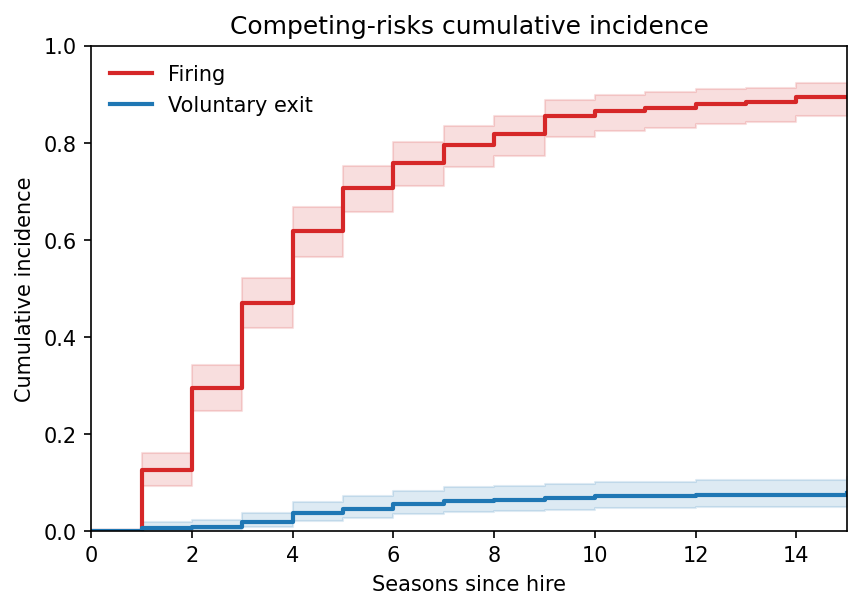
\includegraphics[width=0.75\textwidth]{figures/survival_cif.png}
\caption{Aalen--Johansen cumulative incidence of firing (the event of interest) versus voluntary-while-viable departure (the competing event), with 95\% confidence bands. Firing incidence exceeds voluntary-departure incidence at every horizon.}
\label{fig:cif}
\end{figure}

\subsection{Feature selection}
\label{sec:selection_results}

Cox-native stability selection identifies a single robustly selected predictor. Only the internal-hire indicator clears the $\pi = 0.6$ retention threshold, selected in 82\% of coach-level subsamples (Table~\ref{tab:stability}, Figure~\ref{fig:stability}). The next features form a tier just below the threshold whose membership depends on the per-subsample shortlist length $q$: age at hire, prior-unit yards-per-play efficiency, years as an NFL position coach, and the hiring team's inherited defensive rating each sit between 0.44 and 0.53 at $q = 10$ and rise to between 0.67 and 0.74 at $q = 20$. The internal-hire indicator, by contrast, is selected in 82 to 92\% of subsamples across the whole range of $q$, so its standing does not depend on that choice. Following Section~\ref{sec:selection}, we carry the five highest-frequency features into the reported hazard and prediction models while reading the stable set proper as the one feature that survives the error-controlled threshold. The paired corrected resampled $t$-test (Section~\ref{sec:eval}) finds no difference in concordance between this five-feature set and the larger, cross-validated set described in Section~\ref{sec:selection} ($\Delta C = +0.002$, $p = 0.53$), so the smaller set sacrifices no discrimination.

\begin{table}[!ht]
\caption{Cox-native stability selection (2000 coach-level subsamples). Selection frequency of each leading feature at per-subsample shortlist lengths $q \in \{10, 15, 20\}$, computed from the same subsamples; the retention threshold is $\pi = 0.6$ (primary $q = 10$). Frequencies at or above the threshold are shown in bold. Only the internal-hire indicator clears the threshold across the range of $q$.}
\label{tab:stability}
\small
\begin{tabular}{lccc}
\toprule
Feature & $q = 10$ & $q = 15$ & $q = 20$ \\
\midrule
Internal hire & \textbf{0.82} & \textbf{0.89} & \textbf{0.92} \\
Age at hire & 0.53 & \textbf{0.64} & \textbf{0.74} \\
Prior-unit yards-per-play efficiency & 0.44 & 0.59 & \textbf{0.71} \\
Years as NFL position coach & 0.48 & \textbf{0.60} & \textbf{0.68} \\
Inherited defensive SRS & 0.44 & 0.57 & \textbf{0.67} \\
\bottomrule
\end{tabular}
\end{table}

\begin{figure}[!ht]
\centering

\includegraphics[width=0.85\textwidth]{figures/survival_stability.png}
\caption{Cox-native stability-selection frequencies over 2000 coach-level subsamples (per-subsample shortlist $q = 10$). Only the internal-hire indicator clears the dashed retention threshold ($\pi = 0.6$); the remaining leading features fall just below it, and the four next-highest are carried into the multivariable model alongside it.}
\label{fig:stability}
\end{figure}

\subsection{Predictive performance}
\label{sec:performance}

Table~\ref{tab:bakeoff} reports discrimination for the Cox model and the four robustness benchmarks on the stable feature set. The Cox model attains a Harrell concordance of 0.602 (95\% CI [0.560, 0.645]) and a close Uno concordance of 0.631 (95\% CI [0.511, 0.751]); the agreement of the two point estimates indicates that censoring does not materially distort the concordance. Uno's interval is the wider of the two not because its estimate is uniformly noisier, in most resamples the two track closely, but because its inverse-probability weighting concentrates on the small number of latest firings near each test split's truncation horizon, so in a few small folds the reweighted pair set becomes unstable and inflates the resampling variance. No competing model separates itself from Cox: the parametric and gradient-boosted alternatives differ from it by at most about a hundredth of a concordance point, well within the resampling uncertainty. The proportional-hazards form therefore carries no predictive penalty that the resampling can detect, and we read the models as indistinguishable in discrimination at this resolution, which supports adopting the more interpretable Cox model as primary.

To locate where this discrimination comes from, we compared the full model against a covariate-free null and a series of single-block ablations under the same coach-level resampling protocol (Table~\ref{tab:ablation}). A model with no covariates scores 0.500 by construction. The entire 33-statistic unit-performance block, the football record that hiring processes scrutinize most heavily, does not separate from chance: its concordance is 0.526 (95\% CI [0.480, 0.573]), and the inherited-situation block scores 0.494 ([0.448, 0.539]). Both intervals include 0.500, so neither block is distinguishable from chance. The two structural variables that anchor the final model are individually far more informative: the internal-hire indicator alone reaches 0.564 (95\% CI [0.532, 0.596]) and age at hire alone 0.560 (95\% CI [0.515, 0.604]), both clearing the chance floor and each recovering roughly three-fifths of the distance from chance to the full model's 0.602. A single binary feature, whether the coach was promoted from within, thus discriminates firing better than all thirty-three prior-performance statistics combined. This ablation anticipates the hazard-ratio results below: what predictive signal exists is concentrated in the circumstances of the hire and in a narrow slice of the prior record, not in the statistical record taken as a block.

\begin{table}[!ht]
\caption{Discrimination of single-block and null-model ablations, averaged over the same 50 leakage-free coach-level splits as Table~\ref{tab:bakeoff}. Each row reports a Cox model fit on the indicated feature set alone. The covariate-free null is 0.500 by construction; the full selected model matches the headline 0.602. Intervals use the same Nadeau--Bengio correction for resample overlap as Table~\ref{tab:bakeoff}.}
\label{tab:ablation}
\small
\begin{tabular}{lc}
\toprule
Feature set & Harrell $C$ [95\% CI] \\
\midrule
No covariates (null) & 0.500 [0.500, 0.500] \\
Coach unit performance (33 stats) & 0.526 [0.480, 0.573] \\
Inherited situation (30 features) & 0.494 [0.448, 0.539] \\
Age at hire only & 0.560 [0.515, 0.604] \\
Internal-hire indicator only & 0.564 [0.532, 0.596] \\
Full selected model & 0.602 [0.560, 0.645] \\
\bottomrule
\end{tabular}
\end{table}

\begin{table}[!ht]
\caption{Model comparison on the five-feature stable set, averaged over 50 leakage-free coach-level splits. $C$ = concordance index; 95\% CI Nadeau--Bengio corrected for resample overlap (Section~\ref{sec:eval}). Higher is better; 0.5 is chance.}
\label{tab:bakeoff}
\small
\begin{tabular}{lcc}
\toprule
Model & Harrell $C$ [95\% CI] & Uno $C$ [95\% CI] \\
\midrule
Cox proportional hazards & 0.602 [0.560, 0.645] & 0.631 [0.511, 0.751] \\
Weibull AFT & 0.615 [0.573, 0.657] & 0.643 [0.526, 0.760] \\
Log-normal AFT & 0.615 [0.576, 0.654] & 0.641 [0.525, 0.758] \\
Log-logistic AFT & 0.615 [0.575, 0.654] & 0.640 [0.524, 0.757] \\
XGBoost-AFT & 0.608 [0.567, 0.648] & 0.634 [0.515, 0.753] \\
\bottomrule
\end{tabular}
\end{table}

A concordance near 0.60 carries real but modest signal: presented with two coaches, the model orders their firing times correctly about three in five times. Calibration tells a complementary story. Figure~\ref{fig:calibration} shows the inverse-probability-weighted Brier score by horizon; the integrated Brier score is 0.176 (95\% CI [0.160, 0.191]), comfortably below the 0.25 of an uninformative model. The Brier score is the mean squared error of the predicted survival probabilities, so 0 marks perfect prediction and 0.25 a model that hands every coach the same coin-flip probability; 0.176 is a 30\% reduction in squared error relative to that uninformative baseline (a Brier skill score of about 0.30), so the model's probabilities carry real information while remaining far from deterministic. The figure is read against the dashed 0.25 line: the vertical distance below it at each horizon is the model's probabilistic skill there. That skill is greatest in the first season, where almost no coach has yet been fired and survival is easy to anticipate, and at long horizons, where almost every coach has been; it nearly vanishes in the third and fourth seasons, where the error peaks near 0.25 and firing decisions are most contested and least determined by pre-hire information.

\begin{figure}[!ht]
\centering
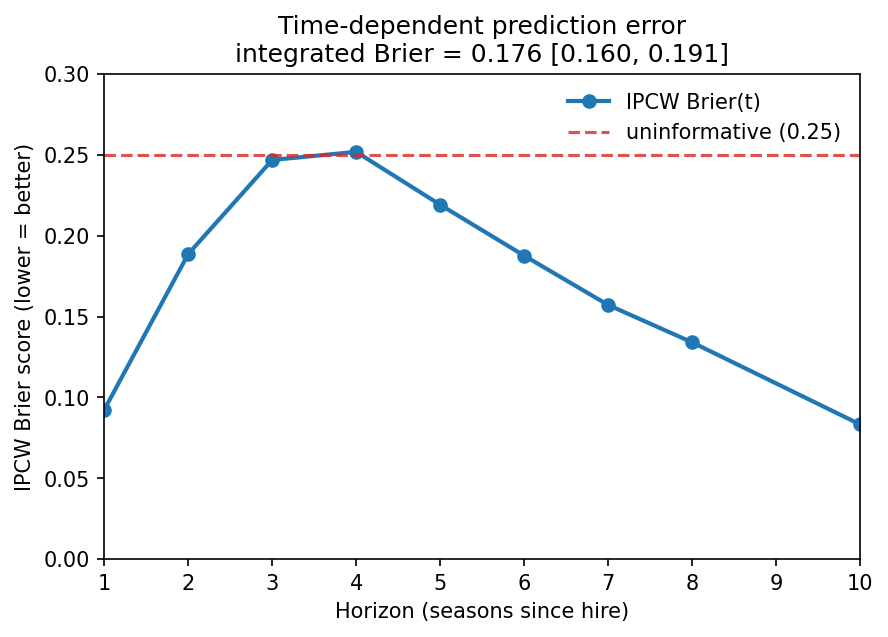
\includegraphics[width=0.7\textwidth]{figures/survival_calibration.png}
\caption{Time-dependent inverse-probability-of-censoring-weighted Brier score for the Cox model by horizon, with the integrated Brier score in the title. Lower is better; the dashed line at 0.25 marks an uninformative model, and the gap below it at each horizon is the model's probabilistic skill there. Error peaks in the contested third and fourth seasons.}
\label{fig:calibration}
\end{figure}

\subsection{Hazard ratios}
\label{sec:hazard}

Table~\ref{tab:hazard} and Figure~\ref{fig:forest} report the cause-specific firing hazard ratios from a Cox model on the five highest-frequency features with cluster-robust standard errors on coach identity. We report this model \emph{without} penalization. With five near-uncorrelated features and 312 events the unpenalized maximum-likelihood fit is stable, and unlike a penalized fit it yields the unbiased coefficients and valid confidence intervals and $p$-values that inference requires. The proportional-hazards assumption is not rejected for any covariate (Grambsch--Therneau minimum $p = 0.20$).

\begin{table}[!ht]
\caption{Cause-specific firing hazard ratios from an unpenalized Cox model on the five highest-frequency features, with cluster-robust standard errors on coach identity. HR $> 1$ indicates faster firing, HR $< 1$ slower. Continuous features are on their natural scale.}
\label{tab:hazard}
\small
\begin{tabular}{lcccc}
\toprule
Feature & HR & 95\% CI & $p$ \\
\midrule
Internal hire & 1.524 & [1.150, 2.021] & 0.003 \\
Age at hire (per year) & 1.021 & [1.003, 1.039] & 0.021 \\
Prior-unit yards-per-play efficiency & 0.739 & [0.614, 0.891] & 0.001 \\
Years as NFL position coach & 1.021 & [0.989, 1.054] & 0.198 \\
Inherited defensive SRS & 1.024 & [0.992, 1.057] & 0.147 \\
\bottomrule
\end{tabular}
\end{table}

\begin{figure}[!ht]
\centering
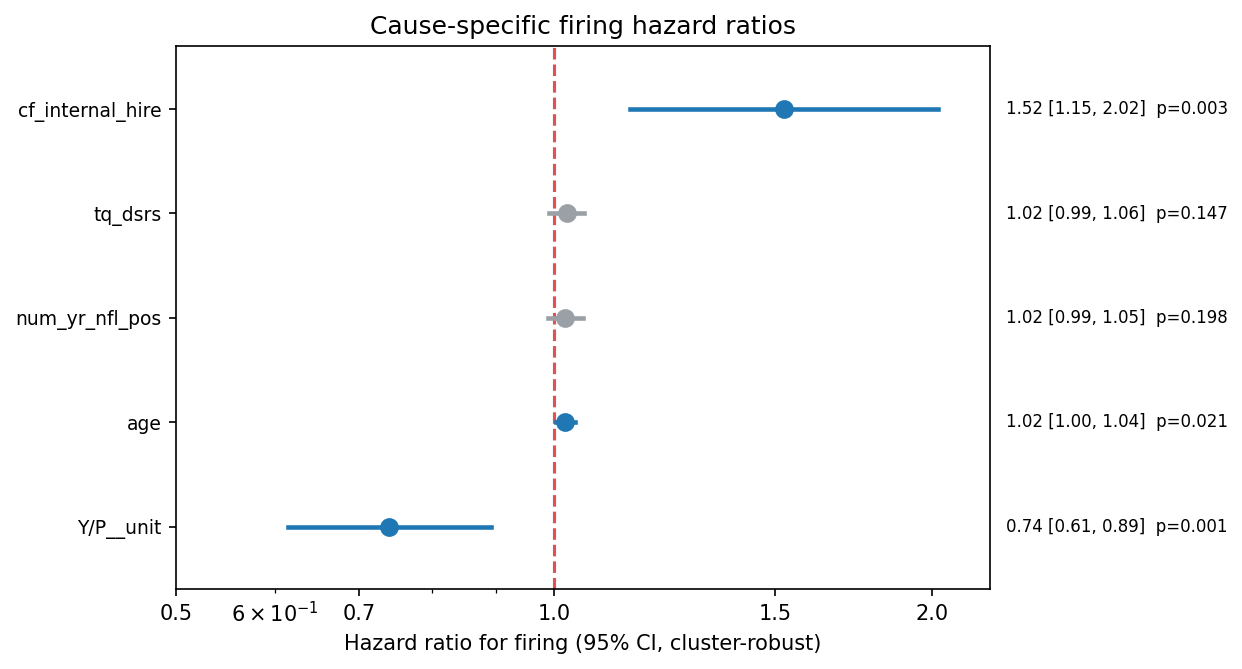
\includegraphics[width=0.85\textwidth]{figures/survival_forest.png}
\caption{Cause-specific firing hazard ratios (unpenalized Cox, cluster-robust 95\% confidence intervals). Significant predictors are shown in blue. The internal-hire indicator, age at hire, and prior-unit yards-per-play efficiency are distinguishable from a hazard ratio of one; the last is protective, a lower hazard for coaches whose prior units gained more yards per play.}
\label{fig:forest}
\end{figure}

Three predictors are distinguishable from a hazard ratio of one. The strongest, and the only feature robustly selected (Section~\ref{sec:selection_results}), is the internal-hire indicator: coaches promoted from within the hiring organization face a markedly higher firing hazard than external hires (HR 1.52, 95\% CI [1.15, 2.02], $p = 0.003$). Two further effects emerge in the multivariable fit. Firing risk rises modestly with age at hire, by about 2\% per year (HR 1.021, 95\% CI [1.003, 1.039], $p = 0.021$), echoing the pattern \citet{farnell2021} report for the broader coaching hierarchy. And coaches whose prior units were more efficient in yards per play face a lower hazard (HR 0.74, 95\% CI [0.61, 0.89], $p = 0.001$), the one slice of the on-field record that carries forward into firing risk, and it does so protectively. The remaining two features, years as an NFL position coach and the inherited defensive rating, have confidence intervals spanning a hazard ratio of one and so cannot be distinguished from no effect in these data. The internal-hire indicator also captures coaches elevated from interim to non-interim status.

The broader pattern across the model is the more important result. Taken as a block, the pooled offensive and defensive unit statistics that make up the largest share of the feature set and that teams scrutinize most heavily discriminate firing at a level indistinguishable from chance (Section~\ref{sec:performance}); their predictive content collapses to a single dimension, yards-per-play efficiency, once the rest of the record is competed away. What foreseeable signal exists is concentrated in how the hire is structured, above all whether the coach is promoted from within rather than brought in from outside, with a thin protective contribution from prior-unit yards-per-play efficiency, rather than in the detailed statistical record.

\section{Discussion}

The analysis yields a connected set of findings. The headline is a ceiling: even with the full pre-hire record in hand, only a modest part of firing is foreseeable. What foreseeable signal exists sits mainly in the structural circumstances of the hire, with a thin protective contribution from the yards-per-play efficiency of the coach's prior units, rather than in the broad on-field record. And dismissal, despite the noise inherent in it, proves a meaningful outcome to model. We develop these in turn, then draw out what they imply for hiring teams and the limits that bound the conclusions.

\subsection{Dismissal is largely unforeseeable at hiring}

The central finding concerns how foreseeable dismissal is in aggregate, more than any single coefficient. With every pre-hire feature available, a calibrated survival model forecasts firing with a concordance near 0.60 and an integrated Brier score of 0.176. This is genuine signal, but a modest one, and it implies that the bulk of what determines a coach's dismissal is not knowable when the contract is signed. The ceiling is a property of the outcome rather than the estimator: the benchmark AFT and gradient-boosted models agree to within sampling error, so it does not move with the choice of model. The interpretation parallels \citet{wolfson2011} on quarterback projection: much of the variation in future success is driven by factors that are simply not observable in advance.

This finding refines, rather than contradicts, the prior literature. \citet{allen2012}, \citet{salaga2020}, and \citet{foreman2019} all show that performance strongly drives dismissal, but they measure performance as it is realized during the tenure, and \citet{allen2012} in particular find that what matters is performance relative to expectations rather than raw results. Our pre-hire analysis speaks to the question those in-tenure studies leave open: the performance that drives firing is largely \emph{not} anticipated by the pre-hire record; teams are not failing to act on a signal they already hold, because most of what will determine the outcome is realized only once the coach is in the role and is not encoded in anything observable on hiring day.

This points to a sharper open question. We have shown that a coach's prior on-field record does not forecast his eventual firing, but we have not tested whether his prior performance \emph{relative to expectations} forecasts his future performance relative to expectations, the quantity the dismissal literature finds decisive. A coach who consistently exceeded the expectations placed on his prior units may carry that tendency forward in a way his raw statistics do not capture. Constructing pre-hire expectation baselines and testing that mapping is a natural direction for future work.

\subsection{Where the foreseeable signal sits}

The clearest pattern in the estimates concerns where the thin signal sits. The internal-hire indicator carries most of it, with the age of the hire and the efficiency of his prior units contributing more weakly, while the bulk of the on-field record and the talent of the inherited roster do not forecast dismissal at all. That the detailed record adds so little is consistent with \citet{roach2016}, who finds that prior head coaching experience does not improve team performance.

To the extent dismissal is foreseeable, the strongest predictor is structural. Promotion from within is associated with a markedly higher firing hazard. The age effect points the same direction, toward the identity and circumstances of the hire. The protective effect of prior-unit efficiency is the one exception, a thread of the on-field record that does carry forward, though it is the weakest of these signals and the least stably selected. For practitioners, the broader implication is that the detailed football credentials given close attention in evaluation have little power to forecast the outcome teams most want to avoid.

The one robust structural signal favors looking outward: external hires survive longer than internal promotions. We are cautious about a causal reading, because internal promotions are bound up with the distressed situations that often produce them, but the pattern is at least consistent with a broader value to outside perspective in a hire. Whether the advantage reflects the outside perspective itself or the healthier circumstances under which external searches are typically conducted is a question our data cannot settle, and a useful one for future work.

\subsection{Dismissal as a meaningful outcome}

A natural concern is whether dismissal is a sensible target at all, given that a coach may be fired for reasons unrelated to quality. Two features of the data support its use. First, dismissal tracks on-field performance in aggregate: as the validity check of Appendix~\ref{app:winrate} shows, mean winning percentage rises across short, medium, and long stints (0.31, 0.41, and 0.54; Kruskal--Wallis $p < 10^{-30}$), so firing is not noise relative to on-field success. Second, by modeling firing specifically and treating voluntary departures as a competing risk, we avoid conflating dismissal with the qualitatively different decision of a successful coach to move on.

\subsection{Implications for hiring and the turnover debate}

These findings have a practical bearing on how teams hire. A coaching search scrutinizes a candidate's prior offenses and defenses and his statistical record closely, yet as a whole that record forecasts firing no better than chance. This is not a case for ignoring the football record, which plausibly bears on performance once a coach is in place, nor against the modest protective signal in prior-unit efficiency; it is evidence that most of the record's predictive content has been competed away by the time a candidate reaches a head-coaching interview, when the league has already sorted candidates on observable competence and little residual variation in pre-hire credentials remains to separate those who will survive from those who will not. What stays foreseeable is largely structural, and the clearest structural factor, the elevated hazard attached to internal and interim-to-non-interim promotions, may reflect the hiring situation as much as the coach: a franchise that promotes from within under duress may be acquiring the distress along with the candidate.

The modest ceiling also speaks to the debate over whether coaching changes accomplish what teams intend \citep{bryson2024}. That coaches exert measurable on-field effects is not in doubt \citep{cannon2025}; what our results bound is not whether coaching matters but how much of a given hire's eventual fate is foreseeable when the contract is signed. If the eventual success of a hire is mostly unwritten on hiring day, the recurring cycle of firing and replacing looks less like the correction of identifiable mistakes than a sequence of draws from a distribution teams cannot fully see in advance. The practical implication is one of calibrated expectations: much of a hire's outcome is uncertain at the time it is made, in the way our calibration results quantify, and a firing that follows need not reflect an identifiable error in the hire.

\subsection{Limitations}

A few limitations qualify these results. The hazard-ratio $p$-values are computed on the same data used to select the features, so they describe the selected model rather than serving as confirmatory tests; the structural predictors, internal hire and age, are theory-motivated and would be included on a priori grounds, which mitigates the concern for them. And the model uses publicly available aggregate statistics; it cannot capture interview performance, leadership, or organizational fit, the kinds of unobservable factors our ceiling result implicates.

\section{Conclusion}

Framing NFL head coach dismissal as a firing-aware, competing-risks survival problem conditioned only on pre-hire information yields a clear picture. Dismissal is only modestly foreseeable at the moment of hiring, the proportional-hazards model is as accurate as more flexible alternatives, and what foreseeable signal exists lies chiefly in the structural circumstances of the hire, above all whether the coach is promoted from within, with weaker contributions from age and from the yards-per-play efficiency of the coach's prior units, rather than in the broad football record that hiring processes emphasize. The same pre-hire, firing-aware question extends naturally to other coaching markets with frequent turnover and a public hiring record, such as Major League Soccer and the NBA \citep{gilfix2020}; whether the modest ceiling we document is particular to the NFL or general to elite coaching labor markets is a question we leave to future work. Coaching changes may be frequent, but at the moment they are set in motion, their eventual outcome is mostly still unwritten.

\noindent\textbf{Reproducibility.}
Data were scraped from Pro-Football-Reference.com. Processed data and analysis code are available at \url{https://github.com/jwilliamson7/CoachingProject} or on request to the corresponding author.

\begin{thebibliography}{99}

\bibitem[Aalen and Johansen(1978)]{aalen1978}
Aalen, O. O. and Johansen, S. (1978). An empirical transition matrix for non-homogeneous Markov chains based on censored observations. \emph{Scandinavian Journal of Statistics}, \textbf{5}(3), pp. 141--150.

\bibitem[Allen and Chadwick(2012)]{allen2012}
Allen, W. D. and Chadwick, C. (2012). Performance, expectations, and managerial dismissal: evidence from the National Football League. \emph{Journal of Sports Economics}, \textbf{13}(4), pp. 337--363.

\bibitem[Austin et al.(2016)]{austin2016}
Austin, P. C., Lee, D. S. and Fine, J. P. (2016). Introduction to the analysis of survival data in the presence of competing risks. \emph{Circulation}, \textbf{133}(6), pp. 601--609.

\bibitem[Brandt(2026)]{brandt2026}
Brandt, A. (2026). Business of football: inside the NFL interview process. \emph{Sports Illustrated}, January 15. Available at \url{https://www.si.com/nfl/business-of-football-inside-nfl-interview-process}.

\bibitem[Bryson et al.(2024)]{bryson2024}
Bryson, A., Buraimo, B., Farnell, A. and Simmons, R. (2024). Special ones? The effect of head coaches on football team performance. \emph{Scottish Journal of Political Economy}, \textbf{71}(3), pp. 295--322.

\bibitem[Cannon et al.(2025)]{cannon2025}
Cannon, A. J., Fisher, J. D., Fellingham, G. W. and Page, G. L. (2025). Analyzing the effects of NBA head coaches. \emph{Journal of Quantitative Analysis in Sports}. DOI: 10.1515/jqas-2025-0025.

\bibitem[Chen and Guestrin(2016)]{chen2016}
Chen, T. and Guestrin, C. (2016). XGBoost: a scalable tree boosting system. In: \emph{KDD '16: Proceedings of the 22nd ACM SIGKDD International Conference on Knowledge Discovery and Data Mining}, pp. 785--794.

\bibitem[Cox(1972)]{cox1972}
Cox, D. R. (1972). Regression models and life-tables. \emph{Journal of the Royal Statistical Society: Series B}, \textbf{34}(2), pp. 187--202.

\bibitem[David et al.(2011)]{david2011}
David, J. A., Pasteur, R. D., Ahmad, M. S. and Janning, M. C. (2011). NFL prediction using committees of artificial neural networks. \emph{Journal of Quantitative Analysis in Sports}, \textbf{7}(2), pp. 1--15.

\bibitem[Davidson-Pilon(2019)]{davidsonpilon2019}
Davidson-Pilon, C. (2019). lifelines: survival analysis in Python. \emph{Journal of Open Source Software}, \textbf{4}(40), 1317.

\bibitem[Farnell et al.(2021)]{farnell2021}
Farnell, A., Berri, D., O'Sullivan, V. and Simmons, R. (2021). Race and coaching hierarchy: an analysis of hiring and firing in the NFL. \emph{Lancaster University Management School, Economics Working Paper Series}, 2021/003.

\bibitem[Fine and Gray(1999)]{finegray1999}
Fine, J. P. and Gray, R. J. (1999). A proportional hazards model for the subdistribution of a competing risk. \emph{Journal of the American Statistical Association}, \textbf{94}(446), pp. 496--509.

\bibitem[Foreman et al.(2019)]{foreman2019}
Foreman, J. J., Soebbing, B. P. and Seifried, C. S. (2019). The impact of deviance on head coach dismissals and implications of a personal conduct policy. \emph{Sport Management Review}, \textbf{22}(4), pp. 491--501.

\bibitem[Gilfix et al.(2020)]{gilfix2020}
Gilfix, Z., Meyerson, J. and Addona, V. (2020). Longevity differences in the tenures of American and foreign Major League Soccer managers. \emph{Journal of Quantitative Analysis in Sports}, \textbf{16}(1), pp. 17--26.

\bibitem[Graf et al.(1999)]{graf1999}
Graf, E., Schmoor, C., Sauerbrei, W. and Schumacher, M. (1999). Assessment and comparison of prognostic classification schemes for survival data. \emph{Statistics in Medicine}, \textbf{18}(17--18), pp. 2529--2545.

\bibitem[Grambsch and Therneau(1994)]{grambsch1994}
Grambsch, P. M. and Therneau, T. M. (1994). Proportional hazards tests and diagnostics based on weighted residuals. \emph{Biometrika}, \textbf{81}(3), pp. 515--526.

\bibitem[Harrell et al.(1996)]{harrell1996}
Harrell, F. E., Lee, K. L. and Mark, D. B. (1996). Multivariable prognostic models: issues in developing models, evaluating assumptions and adequacy, and measuring and reducing errors. \emph{Statistics in Medicine}, \textbf{15}(4), pp. 361--387.

\bibitem[Lin and Wei(1989)]{lin1989}
Lin, D. Y. and Wei, L. J. (1989). The robust inference for the Cox proportional hazards model. \emph{Journal of the American Statistical Association}, \textbf{84}(408), pp. 1074--1078.

\bibitem[Lock and Nettleton(2014)]{lock2014}
Lock, D. and Nettleton, D. (2014). Using random forests to estimate win probability before each play of an NFL game. \emph{Journal of Quantitative Analysis in Sports}, \textbf{10}(2), pp. 197--205.

\bibitem[Meinshausen and B\"uhlmann(2010)]{meinshausen2010}
Meinshausen, N. and B\"uhlmann, P. (2010). Stability selection. \emph{Journal of the Royal Statistical Society: Series B}, \textbf{72}(4), pp. 417--473.

\bibitem[Nadeau and Bengio(2003)]{nadeau2003}
Nadeau, C. and Bengio, Y. (2003). Inference for the generalization error. \emph{Machine Learning}, \textbf{52}(3), pp. 239--281.

\bibitem[Pedregosa et al.(2011)]{pedregosa2011}
Pedregosa, F. et al. (2011). Scikit-learn: machine learning in Python. \emph{Journal of Machine Learning Research}, \textbf{12}, pp. 2825--2830.

\bibitem[Perez(2025)]{perez2025}
Perez, A. J. (2025). How NFL agents spend months scripting coach interviews. \emph{Front Office Sports}, January 15. Available at \url{https://frontofficesports.com/interviews-prep-nfl-head-coaching-candidates/}.

\bibitem[Pro-Football-Reference(2025)]{pfr}
Pro-Football-Reference.com (2025). Pro-Football-Reference. Sports Reference LLC. Available at \url{https://www.pro-football-reference.com/}.

\bibitem[Roach(2016)]{roach2016}
Roach, M. A. (2016). Does prior NFL head coaching experience improve team performance? \emph{Journal of Sport Management}, \textbf{30}(3), pp. 298--311.

\bibitem[Salaga and Juravich(2020)]{salaga2020}
Salaga, S. and Juravich, M. (2020). National Football League head coach race, performance, retention, and dismissal. \emph{Sport Management Review}, \textbf{23}(5), pp. 978--991.

\bibitem[Uno et al.(2011)]{uno2011}
Uno, H., Cai, T., Pencina, M. J., D'Agostino, R. B. and Wei, L. J. (2011). On the C-statistics for evaluating overall adequacy of risk prediction procedures with censored survival data. \emph{Statistics in Medicine}, \textbf{30}(10), pp. 1105--1117.

\bibitem[Wolfson et al.(2011)]{wolfson2011}
Wolfson, J., Addona, V. and Schmicker, R. H. (2011). The quarterback prediction problem: forecasting the performance of college quarterbacks selected in the NFL draft. \emph{Journal of Quantitative Analysis in Sports}, \textbf{7}(3), pp. 1--22.

\end{thebibliography}

\clearpage

\appendix

\section{Feature Descriptions}
\label{app:features}

Table~\ref{tab:featuredefs} defines the pre-hire features outside the pooled unit block, grouped by family; the pooled unit block is described in Section~3.2.1 and its component statistics are itemized in Appendix~\ref{app:unitstats}. All values are measured at or before the hire date.

{\footnotesize
\begin{longtable}{@{}l p{8.6cm}@{}}
\caption{Definitions of the pre-hire features by family. The pooled-unit block is itemized separately in Appendix~\ref{app:unitstats}.}
\label{tab:featuredefs}\\
\toprule
Feature & Definition \\
\midrule
\endfirsthead
\multicolumn{2}{c}{\tablename~\thetable\ (continued)}\\[2pt]
\toprule
Feature & Definition \\
\midrule
\endhead
\midrule
\multicolumn{2}{r}{\footnotesize\itshape continued on next page}\\
\endfoot
\bottomrule
\endlastfoot
\multicolumn{2}{@{}l}{\emph{Core experience (8)}}\\[2pt]
Age at hire & Coach's age in years at the time of hire \\
Prior HC stints & Number of previous head coaching stints \\
College position-coach years & Seasons as a college position coach \\
College coordinator years & Seasons as a college coordinator \\
College head-coach years & Seasons as a college head coach \\
NFL position-coach years & Seasons as an NFL position coach \\
NFL coordinator years & Seasons as an NFL coordinator \\
NFL head-coach years & Seasons as an NFL head coach \\
\addlinespace
\multicolumn{2}{@{}l}{\emph{Career structure (16)}}\\[2pt]
NFL employers & Distinct NFL employers before the hire (relocation-aware) \\
College employers & Distinct college employers before the hire \\
NFL career share & Share of prior coaching seasons spent at the NFL level \\
Age at first job & Age at the coach's first coaching job of any kind \\
Age at first NFL job & Age at the coach's first NFL coaching job \\
Gap before hire & Seasons between the coach's last job and this hire \\
Internal hire & Indicator: promoted from within the hiring organization \\
Years at hiring org & Seasons already spent with the hiring organization before the hire \\
Prior OC & Indicator: ever an offensive coordinator \\
Prior DC & Indicator: ever a defensive coordinator \\
Prior position coach & Indicator: ever a position coach \\
Prior head coach & Indicator: ever a head coach (NFL or college) \\
Prior offensive-side role & Indicator: prior experience on the offensive side of the ball \\
Prior NFL experience & Indicator: any prior NFL-level coaching experience \\
Ever NFL OC & Indicator: ever an NFL offensive coordinator \\
Ever NFL DC & Indicator: ever an NFL defensive coordinator \\
\addlinespace
\multicolumn{2}{@{}l}{\emph{Recent form (5)}}\\[2pt]
Final unit percentile & League percentile of the coach's most recent unit (side-appropriate) in his last ranked season \\
Average unit percentile & Mean league percentile of the coach's units across prior ranked seasons \\
Unit trajectory & Trend in the coach's unit percentile across prior ranked seasons \\
Average team-success percentile & Mean league percentile of team winning percentage across prior ranked seasons \\
Ranked seasons & Number of prior seasons with ranked unit and team data \\
\addlinespace
\multicolumn{2}{@{}l}{\emph{Hiring-team results (3)}}\\[2pt]
Turnovers forced & Turnovers the hiring team forced over its prior two seasons \\
Turnovers committed & Turnovers the hiring team committed over its prior two seasons \\
Playoff appearances & Hiring team's playoff appearances over the prior two seasons \\
\addlinespace
\multicolumn{2}{@{}l}{\emph{Inherited team quality (4)}}\\[2pt]
Offensive SRS & Hiring team's offensive Simple Rating System (points per game vs.\ average, schedule-adjusted) \\
Defensive SRS & Hiring team's defensive Simple Rating System \\
Strength of schedule & SRS strength-of-schedule component faced by the hiring team \\
SRS trajectory & Three-season trend in the hiring team's overall SRS \\
\addlinespace
\multicolumn{2}{@{}l}{\emph{Inherited roster (10)}}\\[2pt]
Starting-QB value & Approximate Value of the inherited starting quarterback \\
Roster value & Total Approximate Value of the inherited roster \\
Starter value & Approximate Value of the inherited starters \\
Starter experience & Mean seasons of experience among inherited starters \\
Roster experience & Mean seasons of experience across the inherited roster \\
Recent first-round picks & First-round draft picks on the inherited roster from recent drafts \\
Premium draft capital & Recent early-round (premium) draft capital on the roster \\
Roster turnover & Share of the roster turned over entering the hire \\
Offensive retention & Offensive personnel retained from the prior season \\
Defensive retention & Defensive personnel retained from the prior season \\
\addlinespace
\multicolumn{2}{@{}l}{\emph{Organizational instability (2)}}\\[2pt]
Predecessor tenure & Seasons the predecessor head coach lasted \\
Head coaches in prior decade & Distinct head coaches the organization employed in the previous ten years \\
\end{longtable}
}

\section{Pooled Unit Statistics}
\label{app:unitstats}

The pooled unit block summarizes a coach's prior on-field production in 33 statistics, each measured for the unit the coach's role controlled and pooled across his qualifying role-seasons as described in Section~3.2.1. For an offensive coordinator a statistic reflects his own offense, for a defensive coordinator the suppression of the opposing offense, and for a head coach his whole team. Every value is standardized against its season's league distribution (Equation~\ref{eq:zscore}) and oriented so that larger is better, with turnovers, interceptions, penalties, and turnover percentage sign-flipped accordingly. Table~\ref{tab:unitstats} lists the 33 statistics in their source order.

{\footnotesize
\begin{longtable}{@{}l l@{}}
\caption{The 33 pooled unit statistics, each standardized by season and oriented so that larger is better. A defensive coordinator's seasons contribute the same quantities measured against the opposing offense.}
\label{tab:unitstats}\\
\toprule
Statistic & Description \\
\midrule
\endfirsthead
\multicolumn{2}{c}{\tablename~\thetable\ (continued)}\\[2pt]
\toprule
Statistic & Description \\
\midrule
\endhead
\midrule
\multicolumn{2}{r}{\footnotesize\itshape continued on next page}\\
\endfoot
\bottomrule
\endlastfoot
Points scored & Points scored by the unit \\
Total yards & Total yards gained \\
Yards per play & Yards gained per offensive play \\
Turnovers & Turnovers committed (sign-flipped) \\
First downs & First downs gained \\
Completions & Pass completions \\
Pass attempts & Pass attempts \\
Passing yards & Yards gained passing \\
Passing touchdowns & Touchdown passes \\
Interceptions & Interceptions thrown (sign-flipped) \\
Net yards per attempt & Net yards per pass attempt, sacks included \\
Passing first downs & First downs gained passing \\
Rush attempts & Rushing attempts \\
Rushing yards & Yards gained rushing \\
Rushing touchdowns & Rushing touchdowns \\
Yards per carry & Yards per rushing attempt \\
Rushing first downs & First downs gained rushing \\
Penalties & Penalties committed (sign-flipped) \\
Penalty yards & Yards lost to penalties (sign-flipped) \\
First downs by penalty & First downs awarded by opponents' penalties \\
Drives & Number of offensive drives \\
Scoring percentage & Share of drives ending in a score \\
Turnover percentage & Share of drives ending in a turnover (sign-flipped) \\
Time per drive & Average time of possession per drive \\
Plays per drive & Average plays per drive \\
Yards per drive & Average yards per drive \\
Points per drive & Average points per drive \\
Third-down attempts & Third-down attempts \\
Third-down rate & Third-down conversion rate \\
Fourth-down attempts & Fourth-down attempts \\
Fourth-down rate & Fourth-down conversion rate \\
Red-zone attempts & Trips inside the opponent's twenty-yard line \\
Red-zone rate & Share of red-zone trips ending in a touchdown \\
\end{longtable}
}

\section{Non-Firing Event Classifications}
\label{app:nonfiring}

Table~\ref{tab:nonfiring} lists every stint coded as a voluntary-while-viable departure, the competing event in our analysis, together with the category assigned under the protocol of Section~\ref{sec:coding} and a one-line justification drawn from contemporaneous reporting. All terminated stints not listed here are coded as involuntary non-retention (firings); the conservative default-to-firing rule means a stint appears below only where positive evidence of a voluntary, while-viable exit was found. The 32 further non-firing stints not shown are coaches still active at the 2025 data boundary, who are administratively censored: Aaron Glenn, Andy Reid, Ben Johnson, Brian Callahan, Brian Daboll, Brian Schottenheimer, Dan Campbell, Dan Quinn, Dave Canales, DeMeco Ryans, Jim Harbaugh, John Harbaugh, Jonathan Gannon, Kellen Moore, Kevin O'Connell, Kevin Stefanski, Kyle Shanahan, Liam Coen, Matt LaFleur, Mike Macdonald, Mike McDaniel, Mike Tomlin, Mike Vrabel, Nick Sirianni, Pete Carroll, Raheem Morris, Sean McDermott, Sean McVay, Sean Payton, Shane Steichen, Todd Bowles, and Zac Taylor. Sean Payton appears here for his current stint and in Table~\ref{tab:nonfiring} for an earlier voluntary departure, the two being distinct stints.

{\footnotesize
\begin{longtable}{@{}l c c c p{5.4cm}@{}}
\caption{The 27 head coaching stints coded as voluntary-while-viable departures (the competing event), grouped by category. Categories follow the protocol of Section~\ref{sec:coding}: (A) departed for another head coaching position while still wanted; (B) retired while still successful and retained; (C) departed for documented health, family, or other non-football reasons. ``Final (W--L)'' is the coach's record in his final season with the team.}
\label{tab:nonfiring}\\
\toprule
Coach & Stint & Final (W--L) & Cat. & Justification \\
\midrule
\endfirsthead
\multicolumn{5}{c}{\tablename~\thetable\ (continued)}\\[2pt]
\toprule
Coach & Stint & Final (W--L) & Cat. & Justification \\
\midrule
\endhead
\midrule
\multicolumn{5}{r}{\footnotesize\itshape continued on next page}\\
\endfoot
\bottomrule
\endlastfoot
\multicolumn{5}{@{}l}{\emph{(A) Departed for another head coaching position while still wanted}}\\[2pt]
Chuck Fairbanks & 1973--1978 & 11--4 & A & Left for the University of Colorado head job \\
Jack Pardee & 1975--1977 & 9--5 & A & Resigned to take the Redskins head job \\
Bobby Ross & 1992--1996 & 8--8 & A & Left for the Lions head job; Chargers wanted to keep him \\
Bill Parcells & 1993--1996 & 11--5 & A & Left in a personnel dispute to take the Jets job \\
Mike Holmgren & 1992--1998 & 11--5 & A & Left for the Seahawks head coach and GM role \\
Al Groh & 2000 & 9--7 & A & Resigned to take the Virginia (alma mater) head job \\
Jon Gruden & 1998--2001 & 10--6 & A & Traded to Tampa Bay; remained a sought-after head coach \\
\midrule
\multicolumn{5}{@{}l}{\emph{(B) Retired while still successful and retained}}\\[2pt]
Paul Brown & 1970--1975 & 11--3 & B & Retired voluntarily on top; named his own successor \\
Sid Gillman & 1974 & 7--7 & B & Retired on top (Coach of the Year); picked his successor \\
Bill Walsh & 1979--1988 & 10--6 & B & Retired days after winning Super Bowl XXIII \\
Jerry Burns & 1986--1991 & 8--8 & B & Announced his own retirement at 64; no pressure \\
Dick Vermeil & 1997--1999 & 13--3 & B & Retired after winning Super Bowl XXXIV \\
Bill Parcells & 1997--1999 & 8--8 & B & Retired on his own terms; Belichick set to succeed \\
Jimmy Johnson & 1996--1999 & 9--7 & B & Retired (burnout); Dolphins would have retained him \\
Dick Vermeil & 2001--2005 & 10--6 & B & Retired on top, still wanted \\
Bill Cowher & 1992--2006 & 8--8 & B & Stepped down after 15 seasons; SB winner the prior year \\
Bill Parcells & 2003--2006 & 9--7 & B & Retired by his own choice; the Cowboys wanted him back \\
Tony Dungy & 2002--2008 & 12--4 & B & Retired on top after a playoff run; picked his successor \\
Bruce Arians & 2019--2021 & 13--4 & B & Stepped down as a SB winner; picked successor Bowles \\
Sean Payton & 2006--2021 & 9--8 & B & Stepped away wanting time off; team would have kept him \\
\midrule
\multicolumn{5}{@{}l}{\emph{(C) Departed for health, family, or other non-football reasons}}\\[2pt]
John Madden & 1970--1978 & 9--7 & C & Retired due to an ulcer and burnout while still wanted \\
Bill Parcells & 1983--1990 & 13--3 & C & Resigned citing health after Super Bowl XXV \\
Joe Gibbs & 1981--1992 & 9--7 & C & Retired for health and family reasons \\
Bobby Ross & 1997--2000 & 5--4 & C & Resigned mid-season citing health (blood clots) \\
Joe Gibbs & 2004--2007 & 9--7 & C & Resigned for family reasons (grandson's illness) \\
Gary Kubiak & 2015--2016 & 9--7 & C & Retired for health reasons (migraine condition) \\
Bruce Arians & 2013--2017 & 8--8 & C & Retired citing family after a 42-year career \\
\end{longtable}
}

\section{Outcome Validity: Win Rate by Tenure Length}
\label{app:winrate}

\begin{figure}[!ht]
\centering
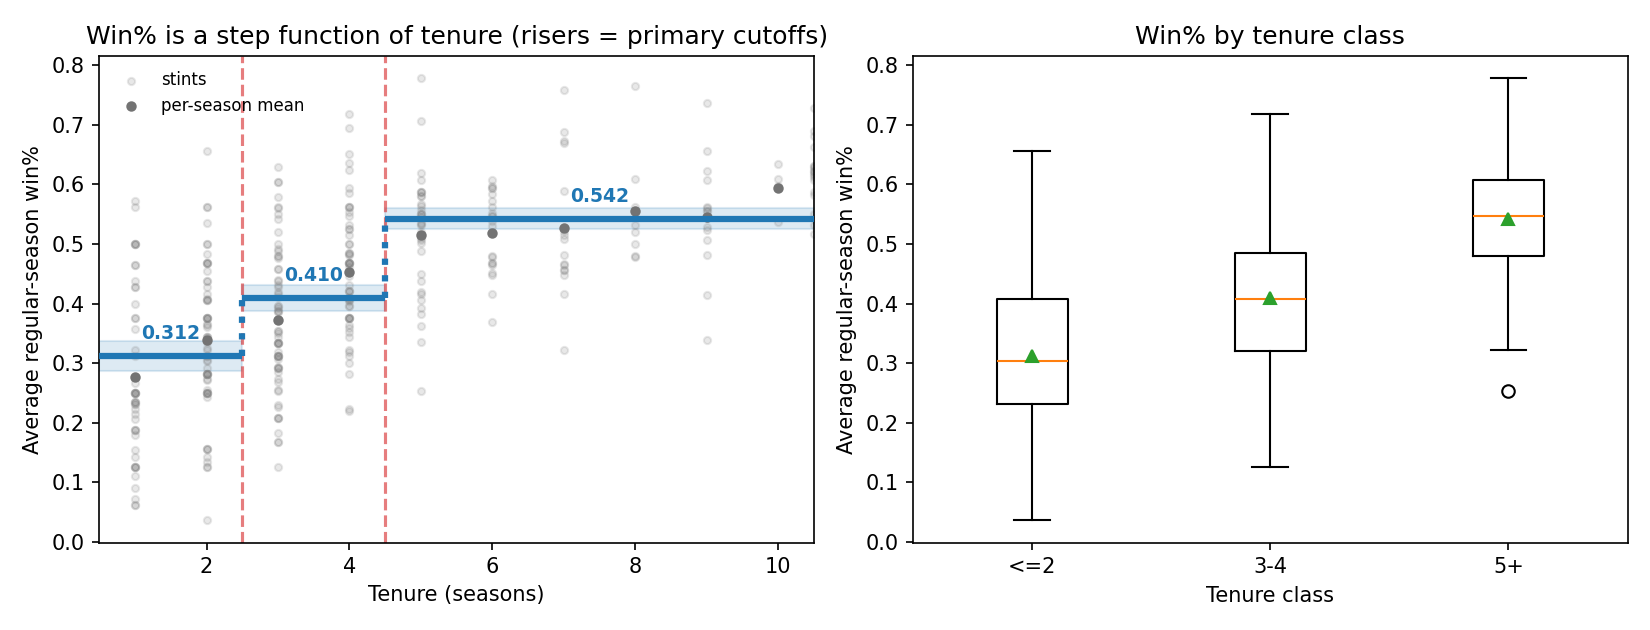
\includegraphics[width=0.75\textwidth]{figures/threshold_winrate.png}
\caption{Mean regular-season winning percentage by tenure length, which rises from 0.31 for short stints to 0.41 for medium and 0.54 for long (Kruskal--Wallis $p < 10^{-30}$; each adjacent step ordered by a one-sided Mann--Whitney test, $p < 10^{-7}$). Dismissal therefore tracks on-field success and is a meaningful outcome to model.}
\label{fig:winrate}
\end{figure}

\section{Model Configuration}
\label{app:hyperparameters}

For predictive evaluation the Cox model uses elastic-net regularization (penalizer $0.5$, $\ell_1$ ratio $0.25$), selected by coach-level cross-validated concordance from an exhaustive grid over penalizer $\in \{0.001, 0.005, 0.01, 0.05, 0.1, 0.3, 0.5, 1.0, 2.0\}$ and $\ell_1$ ratio $\in \{0, 0.25, 0.5, 0.75, 1.0\}$, and held fixed across the 50 resamples. The reported hazard-ratio model (Table~\ref{tab:hazard}) is unpenalized, for the inferential reasons given in Section~\ref{sec:hazard}. Stability selection operates on the 74-feature pool that remains after collapsing groups of highly correlated duplicates to a single representative (Section~\ref{sec:selection}), drawing 2000 coach-level subsamples at 50\% sampling and retaining features with selection frequency at least 0.6 among the top 10 per subsample, with the selection profile also recorded at the top 15 and 20. The XGBoost-AFT benchmark uses a normal AFT loss and was tuned by random search over 200 draws from a grid spanning the number of boosting rounds, learning rate, tree depth (2 to 5), row and column subsampling, minimum child weight, and $\ell_2$ regularization, so that interaction structure up to depth five was available to it; the parametric AFT benchmarks use a small ridge penalty ($0.01$). All resampling uses an 80/20 coach-level train/test split.

\end{document}
